\section{Auswertung}
\label{sec:Auswertung}


\subsection{bestimmung der Apparetekonstante}
\begin{table}[H]
  \begin{minipage}{0.5\linewidth}
    \centering
    \begin{tabular}{c|c}
      \toprule
      {$t_{hoch}\left[\unit{\s}\right]$} & {$t_{runter}\left[\unit{\s}\right]$}\\
      \midrule
      12.85 & 12.97\\
      12.97 & 13.10\\
      13.00 & 12.85\\
      13.00 & 12.94\\
      13.00 & 13.13\\
      13.07 & 13.00\\
      13.05 & 13.03\\
      13.13 & 13.00\\
      12.97 & 13.12\\
      13.03 & 13.12\\
      \bottomrule
    \end{tabular}
    \vspace{5pt}
    \caption{Fallzeiten der kleinen\\ Kugel bei Raumtemperatur}
    \label{table:kk}
  \end{minipage}
  \begin{minipage}{0.5\linewidth}
    \centering
    \begin{tabular}{c|c}
      \toprule
      {$t_{hoch}\left[\unit{\s}\right]$} & {$t_{runter}\left[\unit{\s}\right]$}\\
      \midrule
      52.53 & 52.78\\
      53.19 & 52.38\\
      53.79 & 52.97\\
      53.69 & 53.16\\
      53.53 & 53.19\\
      \bottomrule
    \end{tabular}
    \vspace{5pt}
    \caption{Fallzeiten der großen\\ Kugel bei Raumtemperatur}
    \label{table:gk}
  \end{minipage}
\end{table}

Die mittlere Fallzeit kann mit \ref{eqn:6} berechnet werden.\\
%Gemittelte Fallzeiten kleine Kugel: \qquad \qquad \qquad \qquad Große Kugel:
\begin{align}
  \bar{t}_{\text{hoch}} &= 13.007\,\unit{\second}  \quad &\bar{t}_{\text{hoch}} &= 53.346\,\unit{\second}\\
  \bar{t}_{\text{runter}} &= 13.026\,\unit{\second}  \quad &\bar{t}_{\text{hoch}} &= 52.896\,\unit{\second}\\
  \bar{t}_{\text{gesamt}} &= 13.0165\,\unit{\second}  \quad &\bar{t}_{\text{gesamt}} &= 53.121\,\unit{\second}
\end{align}

Die Dichte der kleinen Kugel mit Gleichung \ref{eqn:4} berechnen:
\begin{equation}
  ρ_{Kl} = \frac{3 \cdot 4.4531 \unit{\gram}}{4 \cdot π \cdot (7.795 \pm 0.01 \unit{\milli\meter})^3} = \SI{2.245(0.009)}{\g\per\cubic\centi\metre}
\end{equation}\label{eqn:13}
\noindent Nun in Gleichung \eqref{eqn:2} einsetzen um die Viskosität von Wasser bei Raumtemperatur zu erhalten.
\begin{equation}
  η = \SI{1.239(0.009)e-06}{\pascal\s}
\end{equation}
Gleichung \ref{eqn:2} nach K umstellen und das Ergebnis von \ref{eqn:13} für $η$ einsetzen
\begin{equation}
  K = \SI{1.673(0.017)e-5}{\pascal\centi\cubic\meter\per\gram}
\end{equation}
\newpage

\subsection{Viskosität in Abhängigkeit der Temperatur}
Um die Konstanten A und B zu ermitteln wird die Gleichung \eqref{eqn:AndradscheGl} umgestellt.
Mithilfe der Python Funktion polyfit werden A und B ermittelt.
\begin{equation}
  \Leftrightarrow ln(η) = ln(\text{A}) + \frac{\text{B}}{\text{T}}
\end{equation}
\begin{equation}
  A = (1792.338 ± 26.764) \quad , \quad B = (-12.822 ± 0.086)\si{\kelvin}
\end{equation}
\begin{figure}[H]
  \centering
  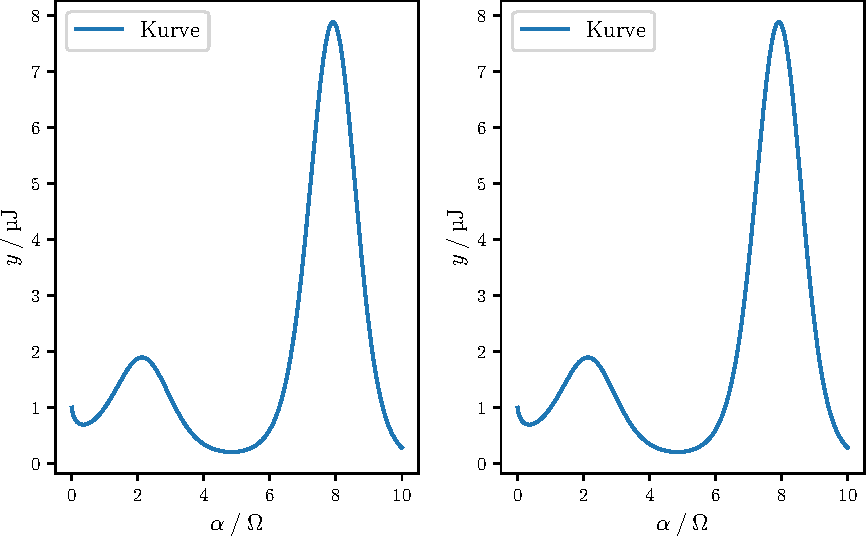
\includegraphics[width=1\textwidth]{build/plot.pdf}
  \caption{Plot der Messdaten und der Regressionskurve\protect\footnotemark}
  \label{fig:plot}
\end{figure}

\begin{table}[!htp]
  \centering
  \begin{tabular}{c|c|c}
    \toprule
    $T [\unit{\degreeCelsius}]$ & $t_{\text{runter}} [\unit{\second}]$ & $t_{\text{hoch}} [\unit{\second}]$\\
    \midrule
    27.5 & 47.5 & 46\\%warum kann ich hier keine Multirow machen?????!!!!?!?!?!
    27.5 & 45 & 43.97\\
    29 & 43.47 & 42.97\\
    29 & 44.13 & 42.81\\
    30.5 & 42.19 & 41.59\\
    30.5 & 42.4 & 41.34\\
    32 & 41.69 & 41.12\\
    32 & 41.91 & 40.66\\
    39.5 & 36.03 & 35.15\\
    39.5 & 35.41 & 35.53\\
    47 & 32.18 & 31.03\\
    47 & 31.66 & 30.79\\
    50 & 30.38 & 29.97\\
    50 & 29.91 & 29.34\\
    52 & 28.63 & 28.22\\
    52 & 28.91 & 28.22\\
    56 & 27.03 & 26.53\\
    56 & 26.88 & 26.85\\
    \bottomrule
  \end{tabular}
  \label{tabellegkt}
  \caption{Fallzeiten der großen Kugel bei steigender Temperatur}
\end{table}
\newpage

\subsection{Berechnung der Reynoldszahl}
Zur berechnung der Reynoldszahl setzen wir in Gleichung \eqref{eqn:5} für $v = \frac{x}{t}$ \: und \: $d = 2r$ ein.
Die Reynoldszahl der großen Kugel bei Raumtemperatur und bei $\SI{56}{\degreeCelsius}$ beträgt
\begin{align}
  Re_{18} &= (2.827 \pm 0.021)\\
  Re_{56} &= (11.21 \pm 0.09)
\end{align} und liegt damit ein gutes Stück unter dem kritischen Wert $R_{Krit} \approx 2300 ,$
die Strömung ist also laminar.\\

\newpage
%Siehe \autoref{fig:plot}!